\section{The Benchmarx Framework}
\label{sec:Benchmarx}

\NOTE{\emph{Length:} 2 p., \emph{Responsible:} Thomas}

\NOTE{Overview of the framework, provided components, approach to tool integration, synchronization dialogues, design and classification of test cases, execution of test cases.}

\begin{figure}[tb!]
	\centering
	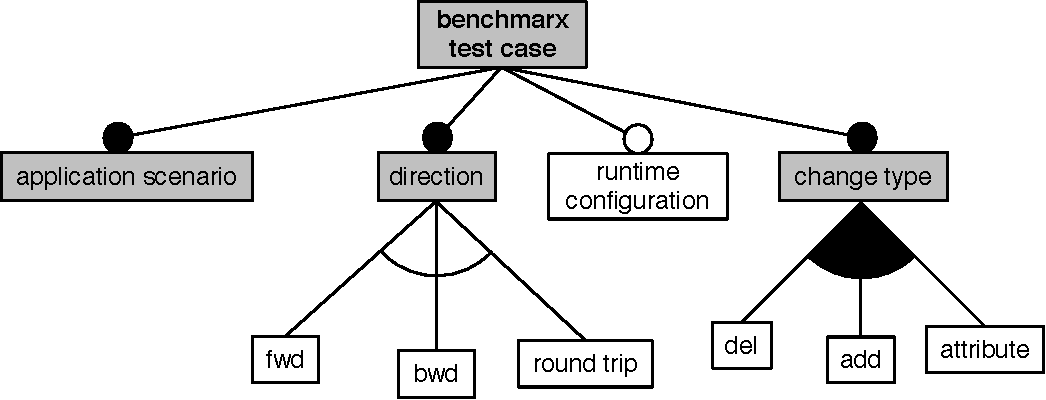
\includegraphics[width=\columnwidth]{diagrams/framework/feature-model-benchmarx-test-case}
	\caption{Variability of benchmarx test cases}
	\label{fig:featureModelBenchmarxTestCase}
\end{figure}

The Benchmarx framework is a component-based framework allowing for 

JUnit-based

no restrictions on the input data of tools

Delta-model

Synchronization Dialogues


